%%%%%%%%%%%%%%%%%%%%%%%%%%%%%%%%%%%%%%%%%%%%%%%%%%%%%%%%%%%%%%%%%%%%%%%%
% Golden Sacra - Memoria
% Escuela Politécnica Superior de la Universidad de Alicante
% Realizado por: Ángel Jesús Terol Martínez
% Contacto: jtm37@alu.ua.es
%%%%%%%%%%%%%%%%%%%%%%%%%%%%%%%%%%%%%%%%%%%%%%%%%%%%%%%%%%%%%%%%%%%%%%%%
\chapter{Manual}
\label{ep:manual}

La \textbf{información} que podemos encontrar por internet acerca de cómo programar en Game Boy puede llegar a ser \textbf{escasa e incluso confusa}. Si bien hay varios tutoriales que ayudan a iniciarse, ninguno llega a explicar con profundidad todos los aspectos. En este apartado veremos lo mejor posible desde \textbf{cómo crear un ejecutable vacío}, a qué \textbf{herramientas} nos pueden ser \textbf{de utilidad} a la hora de empezar un proyecto de estas características:

\section{Creación de una ROM}

Nuestro primer paso será \textbf{crear un ROM vacío} que pueda ser ejecutado en la Game Boy. Esto es muy sencillo de entender y lo básico a la hora de crear un juego.

\begin{lstlisting}[caption={Código base de una ROM}, label={code:baseROM}]
    INCLUDE "hardware.inc"
    
    SECTION	"Cartridge Header",ROM0[$100]
        nop
        jp	Start
        INIT_HEADER

	SECTION "Start",ROM0[$0150]
    Start::
        halt
        jr Start
\end{lstlisting}

Repasemos paso a paso el código. La primera línea \textbf{incluye el fichero de hardware}, el cual contiene todas las direcciones de memoria importantes definidas (dándole un nombre equivalente). No es necesario hacerlo, pero es de gran ayuda a la hora de programar.
\\ \\
En la línea 3 se especifica al programa que, el código que viene justo a continuación, lo debe guardar a partir de la dirección de memoria número \$0100. Como se puede apreciar en la tabla ~\ref{table:4}, es aquí donde se da la \textbf{entrada a la ejecución del programa}. Esto se resume en hacer una pausa y saltar al inicio de nuestro código. En ensamblador esto son \textbf{4 bytes} (\textbf{00 C3 00 01}), con lo que \textbf{la siguiente instrucción se va a guardar} en la posición \textbf{\$0104}, es decir, la \textbf{cabecera del cartucho}.
\clearpage
En la línea 6 tenemos una llamada a una macro, cuya función es definir bytes y \textbf{rellenar las distintas posiciones de memoria que componen la cabecera}:

\begin{lstlisting}[caption={Cabecera del cartucho}, label={code:header}]
INIT_HEADER:	MACRO

	NINTENDO_LOGO

	DB	"GOLDEN SACRA",0,0,0
	DB	$00	; $00 - DMG 
			; $80 - DMG/GBC
			; $C0 - GBC Only cartridge
	DB	$00
	DB	$00
	DB	$00	; $00 - GameBoy Only, $03 - SGB
	DB	CART_ROM_MBC1
	DB	$01	; ROM size, $01 - 512Kbit = 64Kbyte = 4 banks
	DB	$00 ; RAM size
	DB	$01	; $01 - All others
			; $00 - Japan
	DB	$33	; $33 - Check $0144/$0145 for Licensee code.
	DB	$00
	DB	$00
	DW	$00
	
	ENDM
\end{lstlisting}

Su función constiste en llamar, en la línea 4, a otra macro (ya definida dentro del archivo de hardware que se ha incluido previamente) que define \textbf{48 bytes}, los cuales forman el \textbf{bitmap del logo de Nintendo} que aparece nada más encender la Game Boy. Si se altera cualquier byte de los que lo componen, nuestro juego no funcionará en una consola física, ya que el proceso de inicio comprueba que todos sean correctos. Si no lo son, se bloquea.
\\ \\
A continuación tenemos 15 bytes (\textbf{\$0134-\$0143}) para definir el \textbf{título de nuestro videojuego}. Si no llegamos a utilizar todos los carácteres, los espacios sobrantes se rellenan con ceros de forma automática. También lo podemos hacer manualmente, como se muestra en el ejemplo.
\\ \\
El siguiente byte (\textbf{\$0143}) indica si el programa \textbf{soporta funciones especificas de la Game Boy Color}. Con el valor \$80 se puede indicar que sí, pero así además funcionaría en todos los modelos.
\\ \\
Los dos siguientes bytes (\textbf{\$0144-\$0145}) sirven para indicar la \textbf{compañía o la productora del juego}. No es más que un ejemplo así que se va a quedar con valores nulos.
\\ \\
El byte \textbf{\$0146} se utiliza para \textbf{activar o desactivar las funciones SGB}. Estas funciones tienen como objetivo el poder \textbf{conectar una Game Boy a una \textit{SNES}}. Tiene dos valores posibles, \$00 para dejarlas desactivadas o, por el contrario, \$03 para activarlas.
\\ \\
Ahora en el byte \textbf{\$0147} se debe especificar el \textbf{tipo de cartucho}. Si se dejase a valor nulo, diríamos que solo nos interesa aprovechar los 32Kb como ROM. El cartucho \textbf{MBC1}\footnote{\textbf{MBC} son las siglas de \textbf{Memory Bank Controller}. Son chips alojados en la cabecera del cartucho que se utilizan para expandir la memoria mediante la técnica del  \textit{banking}.} seleccionado nos va a permitir un \textbf{máximo de 2Mb como ROM y otros 32Kb como RAM}. Existen \textbf{29 tipos} distintos, y queda a elección del programador elegir cuál utilizar.
\\ \\
Los dos próximos bytes, \textbf{\$0148 y \$0149}, sirven para definir el \textbf{tamaño de la ROM y la RAM}, consecutivamente. En el ejemplo, la ROM ha quedado dividida en 4 bancos (valor \$01). Esto puede ser de gran ayuda a la hora de almacenar música o gráficos. La RAM, por otro lado, se queda en valor nulo ya que se le ha dado un tamaño previo en el tipo de cartucho.
\\ \\
El byte \textbf{\$014A} se utiliza para especificar \textbf{dónde se debe vender el juego}. Las opciones son dos: Japón o cualquier otro país.
\\ \\
El siguiente byte (\textbf{\$014B}) quedó en desuso al poco de sacar nuevos chips. Nuevamente, al igual que los bytes \textbf{\$0144-\$0145}, especificaba la \textbf{compañía o productora}. Sin embargo, \textbf{el valor \$33 significaba que esto ya se había especificado en los bytes nombrados}, por lo que se usaban sus valores en su lugar. Las funciones SGB (si las activamos) no funcionarán si el valor de este byte es distinto de \$33.
\\ \\
Los \textbf{últimos cuatro bytes} (\textbf{\$014D - \$014F}) contienen el \textbf{proceso que comprueba toda la ROM}. El código que ejecuta el primer byte es el siguiente (en C++):

\begin{lstlisting}[caption={Comprobación de la ROM}, label={code:checksum}]
    x=0;
    for(int i=0134h; i < 014Ch; i++){
        x = x-[i]-1;
    }
\end{lstlisting}

\clearpage

Volviendo al \textbf{código~\ref{code:baseROM}}, lo único que resta es poner un \textbf{bucle infinito} para mantener la Game Boy en modo reposo. Si se ejecuta el fichero \textit{.gb} en un emulador o una consola física, el \textbf{resultado} será el siguiente:

\begin{figure}[h]
\centering
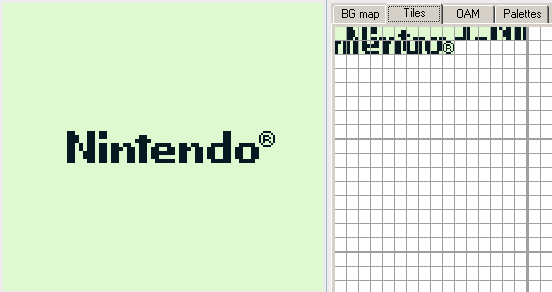
\includegraphics[width=0.7\textwidth]{include/images/VRAM/baseROM.png}
\caption{ROM básica ejecutada en emulador}
\label{figure:baseROM}
\end{figure}

\section{Herramientas}

A la hora de crear un videojuego se necesitan muchos recursos como \textbf{arte o música}. También se necesita de la ayuda de \textbf{librerías que ensamblen y enlacen los distintos ficheros de los que el proyecto se compone}. En esta sección se muestran \textbf{herramientas} que pueden ser de ayuda y cuyo uso es recomendado:

\subsection{RGBDS}

\textbf{RGBDS} (\textbf{Rednex Game Boy Development System}) es una librería gratuita cuya función es \textbf{ensamblar y enlazar los ficheros que componen un proyecto}.
\\ \\
Viene con \textbf{cuatro herramientas}:

\begin{itemize}
	\item \textbf{RGBASM:} Ensamblador.
	\item \textbf{RGBLINK:} Enlazador que creará nuestra ROM.
	\item \textbf{RGBGFX:} Conversor de imágenes .PNG a gráficos de Game Boy. 
	\item \textbf{RGBFIX:} Modificador de la cabecera del cartucho para que cumpla con los requisitos.
\end{itemize}

\clearpage

Para ensamblar y enlazar con la librería se debe ejecutar los siguientes tres comandos en una terminal:

\begin{lstlisting}[caption={Crear una ROM con RGBDS}, label={code:rgbds}]
    rgbasm -ogame.obj game.z80
    rgblink -mgame.map -ngame.sym -ogame.gb game.obj
    rgbfix -p0 -v game.gb
\end{lstlisting}

Pero existe \textbf{un problema}: imagina que el proyecto dispone de 10 ficheros distintos. Ejecutar los \textbf{3 comandos por cada uno} de ellos \textbf{no es viable}. Una solución es crear un fichero \textit{Makefile} para ensamblarlos todos de forma continua y enlazarlos. Un \textbf{ejemplo sencillo} podría ser el que se muestra a continuación:

\begin{lstlisting}[caption={Makefile básico}, label={code:makefile}]
    ASM  = rgbasm
    LINK = rgblink
    FIX  = rgbfix
    MKDIR_P := mkdir -p
    OBJ_DIR := ../obj/
    GB_DIR  := ../
    ROM_NAME = Game_Title
    SOURCES = $(wildcard *.asm)
    FIX_FLAGS = -v -p 0

    OBJECTS = $(SOURCES:%.asm=$(OBJ_DIR)%.o)
    
    all: dirs $(ROM_NAME)
        $(warning Compiled Project)
    
    $(ROM_NAME): $(OBJECTS)
        $(LINK) -o $(GB_DIR)$@.gb -m $(OBJ_DIR)$@.map -n 
            $(OBJ_DIR)$@.sym $(OBJECTS)
        $(FIX) $(FIX_FLAGS) $(GB_DIR)$@.gb
    
    $(OBJ_DIR)%.o: %.asm
        $(ASM) -o $@ $<
    
    clean:
        rm -r $(OBJ_DIR)
        $(warning Cleaned Project)
    
    dirs: 
        $(MKDIR_P) $(OBJ_DIR)
        $(warning Obj Folder Make)
\end{lstlisting}

\clearpage

\subsection{GBTD y GBMB}

\textbf{GBTD} (\textbf{Game Boy Tile Designer}) y \textbf{GBMB} (\textbf{Game Boy Map Builder}) son unos programas gratuitos con los cuales podremos crear nuestros tiles y tilemaps, ambos \textbf{desarrollados por Harry Mulder}. Además, son programas que exportan directamente al lenguaje ensamblador compatible con RGBDS.
\\ \\
El primer programa, \textbf{GBTD}, tiene como utilidad \textbf{la creación de tiles} de diferentes tamaños (8x8, 8x16, 16x16...), tanto con los colores de la Game Boy original como los de la SGB y Game Boy Color.

\begin{figure}[h]
\centering
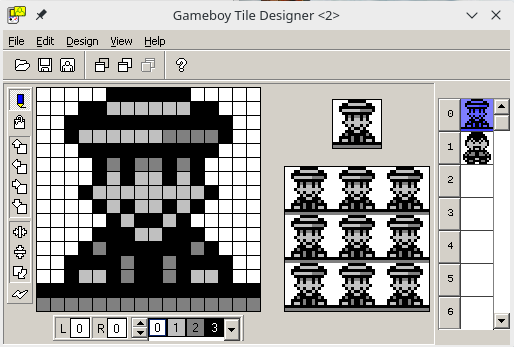
\includegraphics[width=0.5\textwidth]{include/images/manual/gbtd.png}
\caption{Game Boy Tile Designer}
\label{figure:gbtd}
\end{figure}

Por otro lado, con \textbf{GBMB} podremos utilizar los ficheros generados por el GBTD y crear distintos tilemaps, con un tamaño máximo de 1024x1024 píxeles. Además, se puede importar cualquier tile que GBTD soporte.

\begin{figure}[h]
\centering
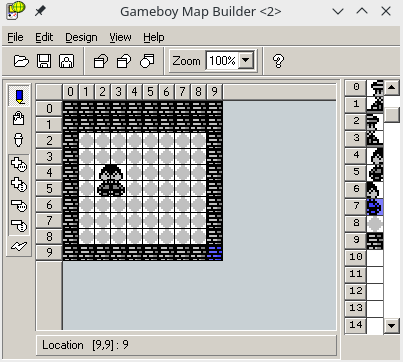
\includegraphics[width=0.5\textwidth]{include/images/manual/gbmb.png}
\caption{Game Boy Map Builder}
\label{figure:gbmb}
\end{figure}

\clearpage

\subsection{Emuladores}

Existen diversos emuladores con los que podemos probar a la perfección nuestros juegos de GB. Sin embargo, \textbf{pocos son los que traen un debugger} con los que podamos visualizar en todo momento lo que está ocurriendo con la memoria.
\\ \\
La mejor opción es el uso de \textbf{BGB}. Permite emular juegos de GB, SGB y GBC. Cuenta con \textbf{muchas herramientas} con las que mejorar el gameplay y, además, es \textbf{muy preciso} a la hora de emular, por lo que cualquier juego que funcione bien aquí también lo hará en una Game Boy real.

\begin{figure}[h]
\centering
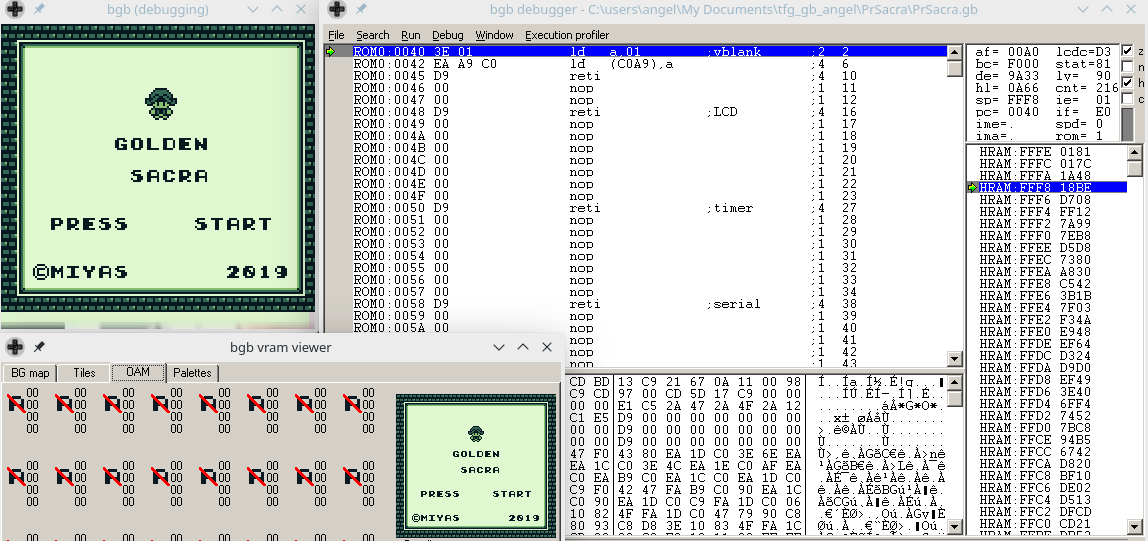
\includegraphics[width=0.9\textwidth]{include/images/manual/bgb.png}
\caption{Emulador BGB}
\label{figure:bgb}
\end{figure}

\textbf{Otro emulador} que podemos usar de manera complementaria es \textbf{NO\$GMB}. Su \textbf{debugger} es \textbf{más cómodo} de utilizar, pero existen diferencias cruciales entre el funcionamiento esperado y el resultado. Existen \textbf{problemas en la emulación del intervalo V-Blank}, por lo que al usarlo en una Game Boy física puede que se den corrupciones del bus de datos.

\begin{figure}[h]
\centering
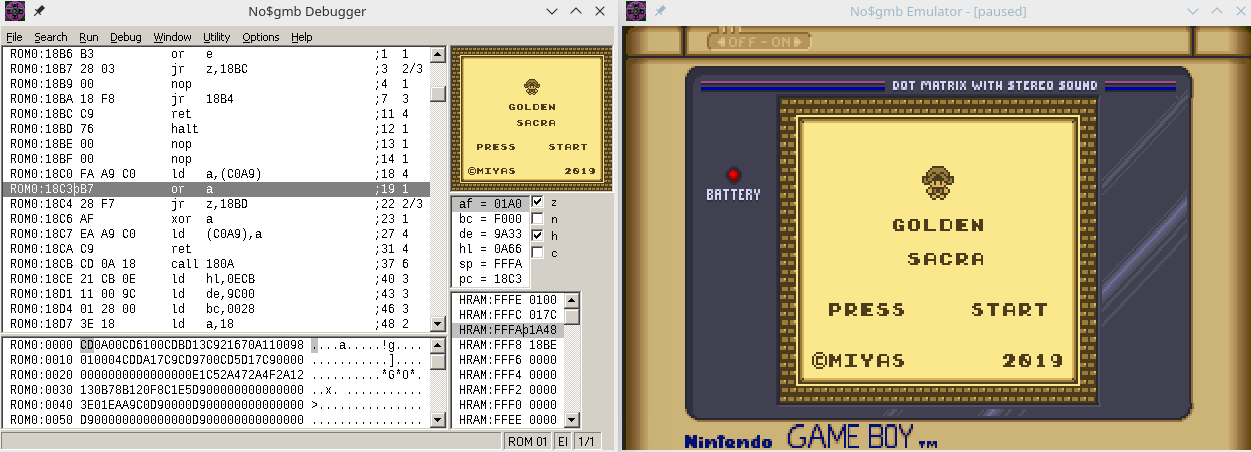
\includegraphics[width=0.9\textwidth]{include/images/manual/nogmb.png}
\caption{Emulador NO\$GMB}
\label{figure:bgb}
\end{figure}

\subsection{Flash Cartridge}

La mejor opción para \textbf{estar completamente seguros de que nuestro juego funciona es probarlo en una Game Boy física}. Para ello tendremos que hacer uso de un \textbf{cartucho flash}, al cual podemos \textbf{introducir ROM's} de diversos juegos. No todo el mundo se lo puede permitir, pero puede resultar de lo más útil.

\begin{figure}[h]
\centering
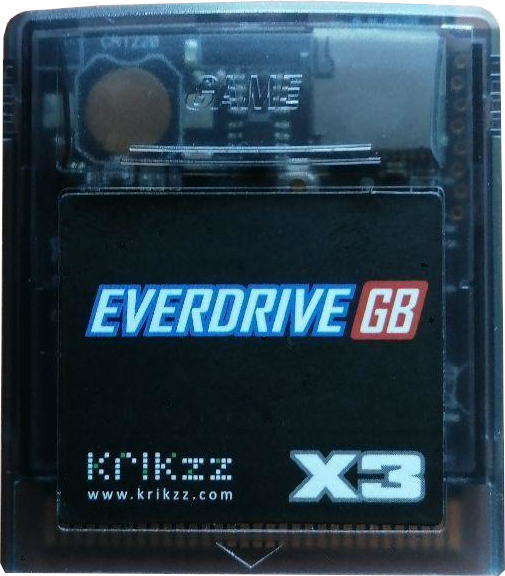
\includegraphics[width=0.2\textwidth]{include/images/manual/flashc.png}
\caption{Game Boy Flash Cartridge}
\label{figure:flashc}
\end{figure}

El \textit{Everdrive} que se muestra en la imagen es el \textbf{modelo más barato} (hablamos alrededor de los 60€), pero funciona perfectamente. Nos permite guardar nuestras partidas y utilizarla en cualquier modelo de Game Boy. Además, \textbf{dispone de todos los \textit{mappers}}, lo cual significa que, asignemos el tipo de cartucho que asignemos en la cabecera de la ROM, vamos a poder hacer uso de él.
\\ \\ 
A la hora de comprar uno, lo único \textbf{necesario es descargar}, desde la página web que se muestra en el propio cartucho, \textbf{los \textit{drivers}} que el fabricante nos marca. 

\subsection{GBSound Sample Generator}
\label{GBSound}
\textbf{GBSound Sample Generator} es un programa que podemos ejecutar tanto en emulador como en hardware real, \textbf{bastante sencillo de usar}, en el que podemos modificar los valores de los registros de sonido y probar directamente su resultado.

\begin{figure}[h]
\centering
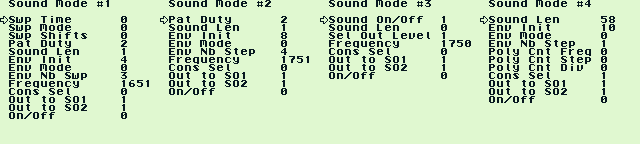
\includegraphics[width=1\textwidth]{include/images/manual/gbsound.png}
\caption{GBSound Sample Generator}
\label{figure:gbsound}
\end{figure}

En vez de establecer el valor bruto de los registros en el código, \textbf{definiremos una frecuencia de sonido, un nivel de volumen, una envolvente, un ciclo de trabajo, etc}. Como los valores se muestran por pantalla, si queremos reproducir ese sonido exacto \textbf{solamente tendremos que copiar los 3 o 4 bytes que el programa nos da}.

\clearpage

\subsection{Sublime Text 3}

Por último, vamos a utilizar como editor de texto \textbf{Sublime Text 3}. Es una herramienta muy \textbf{sencilla, ligera y con un abanico de comandos muy extenso}. 
\\ \\
La \textbf{interfaz gráfica} consta de una \textbf{barra lateral izquierda}, donde se muestra el \textbf{sistema de ficheros}, comenzando desde la carpeta raíz que se haya indicado, y una \textbf{barra lateral derecha} donde se encuentra una \textbf{copia del documento, pero en forma de slider y en miniatura}. Este último es muy útil a la hora de navegar por el documento.
\\ \\
Además, tiene la opción de \textbf{instalar paquetes} que añadan funcionalidades al editor. Estos paquetes pueden ser descargados de otros usuarios o, por el contrario, programados. Para estre proyecto se recomienta instalar el paquete de \textbf{RGBDS}, el cual se va a encargar de pintar cada palabra de un color, según la sintaxis indicada por el propio ensamblador.

\begin{figure}[h]
\centering
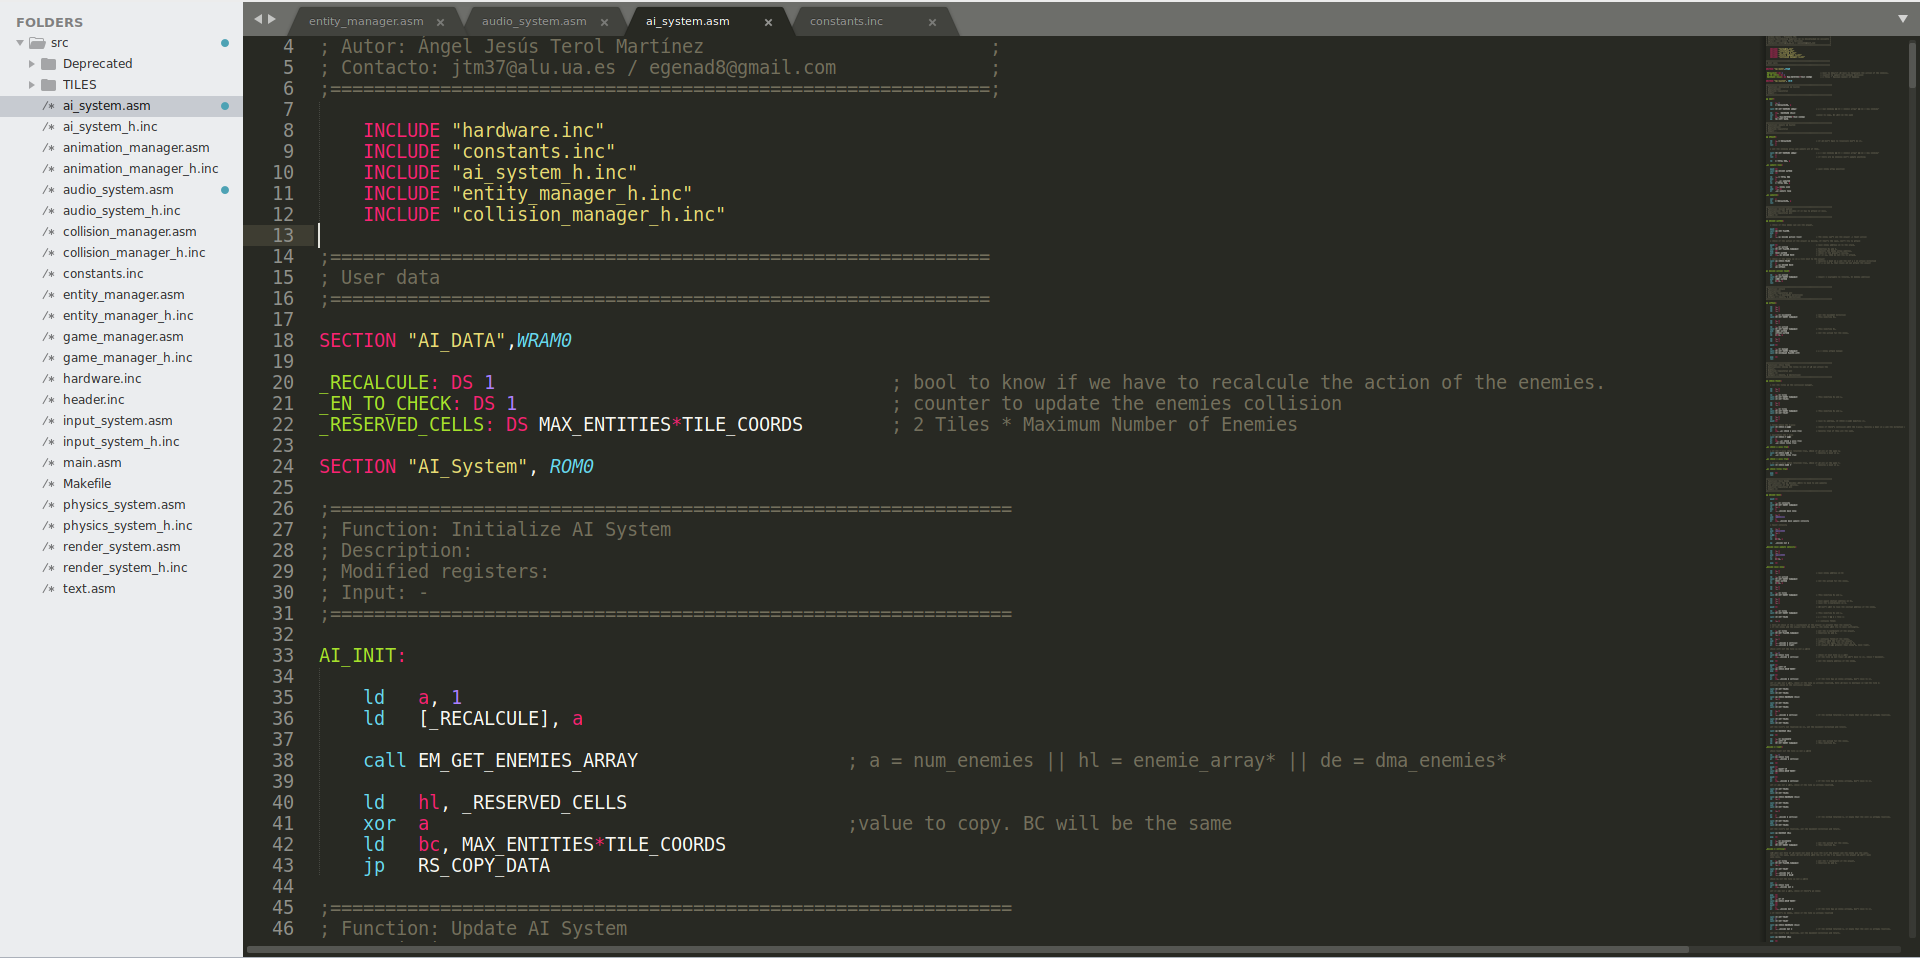
\includegraphics[width=1\textwidth]{include/images/manual/sublime.png}
\caption{Interfaz Sublime Text 3}
\label{figure:sublime}
\end{figure}

\clearpage

\section{Tiles}

Ya se han mencionado y visto como generarlos usando distintas herramientas pero, ¿conocemos en detalle realmente qué son o cómo funcionan?
\\ \\
La primera diferencia a tener en cuenta es que \textbf{un tile no es un sprite}. Se puede afirmar, sin embargo, que \textbf{los sprites están compuestos por un tile} (como mínimo). 
\\ \\
Así pues, un tile es \textbf{conjunto de píxeles} que, de manera general, forman un tamaño de 8x8. Para utilizarlos en un proyecto, lo primero que se debe hacer es incluirlos (después de haberlos generado con la herramienta GBMB):

\begin{lstlisting}[caption={Inclusión de un Fichero Binario}, label={code:tiles}]
SECTION "Tiles", ROM0
Tiles:
	INCLUDE "./TILES/tilemap.z80"
Fin_tiles:
\end{lstlisting}

\textbf{La Game Boy funciona por ``capas''}, donde cada una se dibuja por encima de la anterior. Como se ha podido ver, existen 2 fondos de pantalla sobre los cuales dibujar tiles. La \textbf{pantalla principal} es la que sirve de \textbf{fondo} (árboles, casas, ríos... Cualquier cosa que no vaya a necesitar actualizarse constantemente). La \textbf{segunda pantalla}, la cual se puede esconder, se utiliza de forma común para el \textbf{HUD} (ventanas emergentes del inventario o guardado, por ejemplo). La \textbf{tercera capa} es la de los \textbf{sprites}. En esta última capa es donde va a estar el personaje, enemigos, etc.

\begin{figure}[h]
\centering
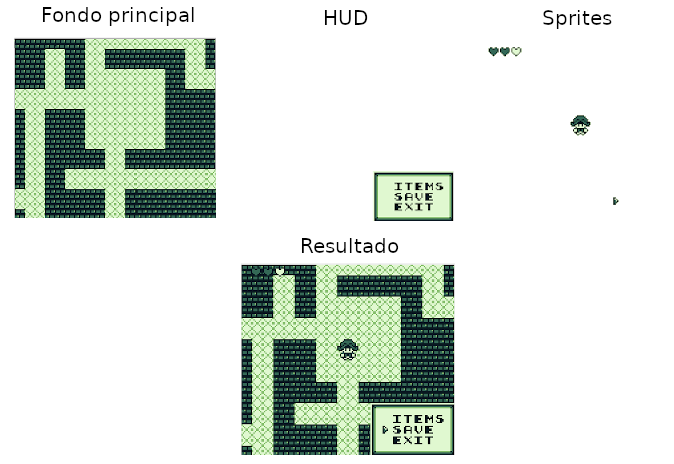
\includegraphics[width=0.8\textwidth]{include/images/manual/capas.png}
\caption{Capas de la Game Boy}
\label{figure:bgb}
\end{figure}

\clearpage

\section{Sprites}
\label{manual_sprites}

Sabemos diferenciarlos de los tiles y cómo podemos generarlos. Lo único que falta por conocer es el \textbf{cómo se estructuran en memoria}.
\\ \\
Los sprites se almacenan en el \textbf{Object Array Memory} (\textbf{OAM}), y \textbf{ocupan siempre 4 bytes cada uno}. El primer byte es la posición Y, el segundo la posición X, el tercero el número de tile y el cuarto el atributo (que veremos más en detalle).
\\ \\
Lo que se llega a visualizar en memoria una vez se ha creado (como mínimo) un sprite, es un \textbf{vector de bytes}. Estos valores se deberán saber diferenciar empezando desde la primera posición de todas. A continuación se expone una \textbf{representación gráfica}:

\begin{figure}[h]
\centering
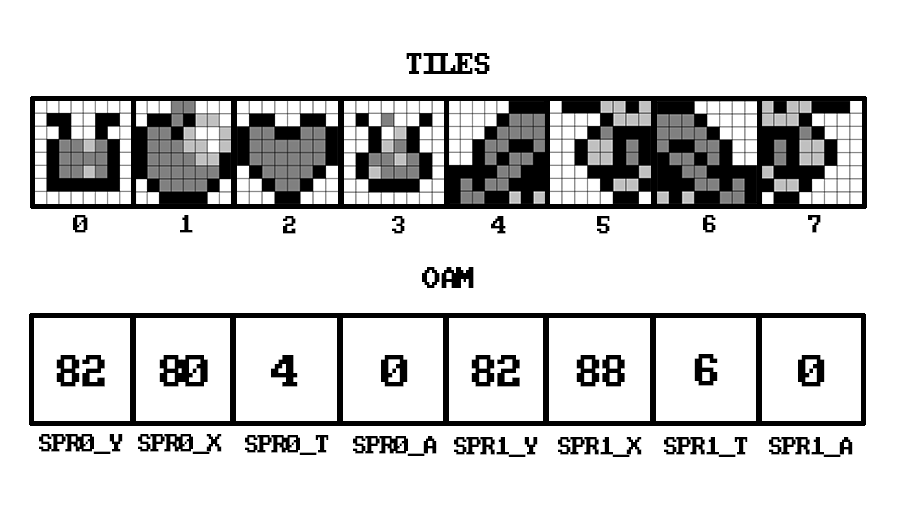
\includegraphics[width=0.7\textwidth]{include/images/manual/sprites_oam.png}
\caption{Descripción Gráfica de la OAM}
\label{figure:spr_oam}
\end{figure}

Los bytes de la OAM que se representan en la imagen darían como resultado \textbf{media cabeza de un personaje}, puesto que el primero tiene indicado que muestre el tile número 4 y el segundo el número 6. Remarcar que \textbf{ambos sprites se separan por 8 píxeles en el eje X}, el cual es el ancho de un tile.

\cleardoublepage %salta a nueva página impar




